\documentclass[11pt, a4paper]{article}
\usepackage{amsmath}
\usepackage{amssymb}
\usepackage{enumitem}
\usepackage{graphicx}
\usepackage{fullpage}
\usepackage[colorlinks=true, linkcolor=blue]{hyperref}
\usepackage{subfigure}
\usepackage{url}

\renewcommand{\arraystretch}{1.25} % line spacing in tabular environment
\addtolength{\jot}{0.1em} % line spacing in align environment
\newcommand{\R}{\mathbb{R}}

\begin{document}
\title{COMP4680: Advanced Topics in Statistical Machine Learning\\Second Programming Assignment}
\author{Libo Yin (u5483742)\\The Australian National University}
\maketitle

\section{Probabilistic Filtering on a Hidden Markov Model}

\begin{enumerate}[topsep=0em, itemsep=-1ex, partopsep=1ex, parsep=1ex, label=(\alph*)]
\item
\begin{align*}
&P(x_0, x_1, \ldots, x_t, y_1, \ldots, y_t)\\
&=P(x_0, x_1, \ldots, x_t, y_1, \ldots, y_{t-1})P(y_t|x_0, x_1, \ldots, x_t, y_1, \ldots, y_{t-1})\\
&\quad\text{note that }y_t\perp\{x_0, x_1, \ldots, x_{t-1}, y_1, \ldots, y_{t-1}\}|x_t\\
&=P(x_0, x_1, \ldots, x_t, y_1, \ldots, y_{t-1})P(y_t|x_t)\\
&=P(x_0, x_1, \ldots, x_{t-1}, y_1, \ldots, y_{t-1})P(x_t|x_0, x_1, \ldots, x_{t-1}, y_1, \ldots, y_{t-1})P(y_t|x_t)\\
&\quad\text{note that }x_t\perp\{x_0, x_1, \ldots, x_{t-2}, y_1, \ldots, y_{t-1}\}|x_{t-1}\\
&=P(x_0, x_1, \ldots, x_{t-1}, y_1, \ldots, y_{t-1})P(x_t|x_{t-1})P(y_t|x_t)\\
&=\ldots\\
&=P(x_0)\prod_{i=1}^t P(x_i|x_{i-1})P(y_i|x_i)
\end{align*}
\item
\begin{align*}
P(x_t|y_1, \ldots, y_{t-1})&=\int P(x_t, x_{t-1}|y_1, \ldots, y_{t-1})dx_{x-1}\\
&=\int P(x_t|x_{t-1}, y_1, \ldots, y_{t-1})P(x_{t-1}|y_1, \ldots, y_{t-1})dx_{x-1}\\
&\quad\text{note that }x_t\perp\{y_1, \ldots, y_{t-1}\}|x_{t-1}\\
&=\int P(x_t|x_{t-1})P(x_{t-1}|y_1, \ldots, y_{t-1})dx_{x-1}
\end{align*}
\item
\begin{align*}
P(x_t|y_1, \ldots, y_{t-1}, y_t)&=\dfrac{P(x_t, y_t|y_1, \ldots, y_{t-1})}{P(y_t|y_1, \ldots, y_{t-1})}\\
&=\dfrac{P(x_t, y_t|y_1, \ldots, y_{t-1})}{\int P(x_t, y_t|y_1, \ldots, y_{t-1})dx_t}\\
&=\dfrac{P(y_t|x_t)P(x_t|y_1, \ldots, y_{t-1})}{\int P(y_t|x_t)P(x_t|y_1, \ldots, y_{t-1})dx_t}
\end{align*}
\item With $P(y_t|x_t)$ and $P(x_t|x_{t-1})$ known, and $P(x_t|y_1, \ldots, y_t)$ denoted by $f(t),$ we wish to represent $f(t)$ as a function of $f(t-1).$
\begin{align*}
f(t)&=P(x_t|y_1, \ldots, y_t)\\
&=\dfrac{P(y_t|x_t)P(x_t|y_1, \ldots, y_{t-1})}{\int P(y_t|x_t)P(x_t|y_1, \ldots, y_{t-1})dx_t}\\
&=\dfrac{P(y_t|x_t)\int P(x_t|x_{t-1})P(x_{t-1}|y_1, \ldots, y_{t-1})dx_{x-1}}{\int P(y_t|x_t)\int P(x_t|x_{t-1})P(x_{t-1}|y_1, \ldots, y_{t-1})dx_{x-1}dx_t}\\
&=\dfrac{P(y_t|x_t)\int P(x_t|x_{t-1})f(t-1)dx_{x-1}}{\int P(y_t|x_t)\int P(x_t|x_{t-1})f(t-1)dx_{x-1}dx_t}
\end{align*}
\end{enumerate}

\section{Robot Localisation: Particle Filter}

The derivation of Bayesian localization is shown as follows:
\begin{align*}
P(x_t|u_{1:t}, y_{1:t})&=\dfrac{P(x_t, y_t|u_{1:t}, y_{1:t-1})}{P(y_t|u_{1:t}, y_{1:t-1})}\\
&=\dfrac{P(y_t|x_t, u_{1:t}, y_{1:t-1})}{P(y_t|u_{1:t}, y_{1:t-1})}\\
&\quad\text{since the denominator }P(y_t|u_{1:t}, y_{1:t-1})\text{ is a constant wrt }x\\
&\propto P(y_t|x_t, u_{1:t}, y_{1:t-1})P(x_t|u_{1:t}, y_{1:t-1})\\
&=P(y_t|x_t)P(x_t|u_{1:t}, y_{1:t-1})\\
&=P(y_t|x_t)\int P(x_t|x_{t-1},u_{1:t}, y_{1:t-1})P(x_{t-1}|u_{1:t}, y_{1:t-1})dx_{t-1}\\
&=P(y_t|x_t)\int P(x_t|x_{t-1},u_t)\underbrace{P(x_{t-1}|u_{1:t-1}, y_{1:t-1})}_{\text{recursion}}dx_{t-1}
\end{align*}

The last equation clearly demonstrates the correspondence between the continuous but intractable Bayesian localization and particle filtering. Before proposing the motion model $P(x_t|x_{t-1},u_t)$ and the measurement model $P(y_t|x_t)$ for the algorithm, we define $x_t,\ u_t,$ and $y_t:$
\begin{align*}
x_t&=[x:\text{x-coordinate}, y:\text{y-coordinate}, \theta:\text{heading}]^T\in\R^3\\
u_t&=[s:\text{linear motion (odometry)}, \Delta\theta:\text{angular motion}]^T\in\R^2\\
y_t&=[\operatorname{dist}(\bar{x}_t, \beta):\text{observed distance at each bearing }\beta]^T\in\R^{11}
\end{align*}

Since an exact motion model $P(x_t|x_{t-1},u_t)$ is neither given nor needed in particle filtering, we represent the motion model with a sampling model, in which we assume that the linear motion $s$ contains noise $\Delta s$ that follows $N(\mu=0, \sigma=1),$ and the angular motion $\Delta\theta$ is itself a noise that follows $N(\mu=0, \sigma=\pi/4).$
\[P(x_t|x_{t-1},u_t)=P(||x_t-x_{t-1}||;N(\mu=s, \sigma=1))P(x_t^{[\theta]};N(\mu=x_{t-1}^{[\theta]}, \sigma=\pi/4))\]

where $x_t^{[\theta]}$ and $x_{t-1}^{[\theta]}$ denote the heading $\theta$ of a particle at time $t$ and $t-1,$ respectively. For the measurement model $P(y_t|x_t),$ we propose the likelihood of observing $y_t$ given $x_t$ under the measurement noise model $N(\mu=\operatorname{dist}(x_t, \beta), \sigma=1)$ at all 11 bearing angels, which are assumed to be independent. Note that $\operatorname{dist}(x_t, \beta)$ here denotes the ``real distance'', as opposed to the observed distance $\operatorname{dist}(\bar{x}_t, \beta)$ mentioned earlier.


\begin{align*}
P(y_t|x_t)&=\prod_{\beta}\left[
    \begin{array}{l}
    \alpha_{\text{normal}}\\
    \alpha_{\text{max}}\\
    \alpha_{\text{failure}}
    \end{array}
\right]\cdot\left[
    \begin{array}{c}
    P\left(y_t^{[\beta]}; N(\mu=\operatorname{dist}(x_t, \beta), \sigma=1)\right)\\
    1\\
    0
    \end{array}
\right]\\
&\quad\text{where }\sum_\alpha=1,\text{ and }y_t^{[\beta]}\text{ denotes the observed distance at bearing }\beta\\
&\approx\prod_{\beta}P\left(y_t^{[\beta]}; N(\mu=\operatorname{dist}(x_t, \beta), \sigma=1)\right)
\end{align*}

Since this likelihood often gets unstably small (at the magnitude of $10^{-50}$ to $10^{-200}$), we use the inverse negative log likelihood in practice. It is defined as:
\[P\,'(y_t|x_t)=-\frac{1}{P(y_t|x_t)}\]

After the transformation, most weights are at the magnitude of $10^{-2}$ to $10^{-4}.$ However, this also means that the variance of the probability space is significantly reduced. As a result, we employ the low variance sampling algorithm for particle resampling. Note that although the distribution of particles essentially resembles the probability distribution $P(x_t|u_{1:t}, y_{1:t}),$ there is no need to normalize the weight of each particle such that they add up to 1, since such process is implicitly built into the sampling algorithm.

In order to reconstruct the most likely trajectory, each particle maintains a list to keep record of its historical locations and weights. When the main loop of the particle filter has finished, we calculate the likelihood of each trajectory by multiplying all its historical weights. Again, due to possible underflow, this likelihood is calculated in logarithmic form. Finally, we simply choose the trajectory whose history has the highest likelihood.

The trajectory map for scenario ``easy'' and ``hard'' are shown in \hyperref[fig:easy]{figure~\ref{fig:easy}} and \hyperref[fig:hard]{figure~\ref{fig:hard}}. Note that scenario ``hard'' generated two highly symmetrical trajectories. Their heatmap animations are available at \url{http://goo.gl/Pvgkgo}.

\begin{figure}[htbp]
\centering
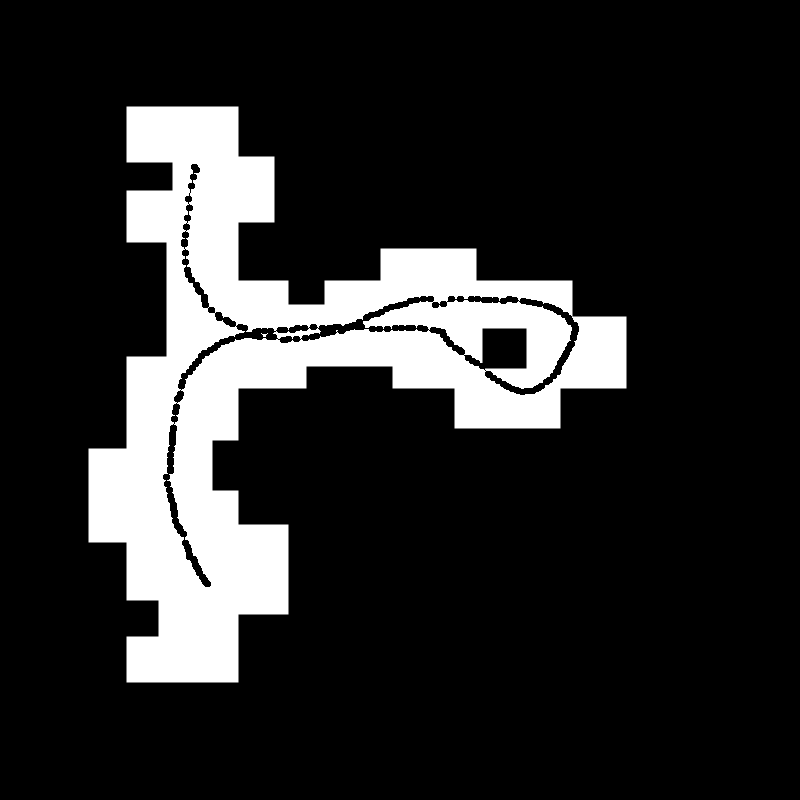
\includegraphics[scale=0.4]{easy.png}
\caption{The most likely trajectory in scenario ``easy'' from 5000 particle trajectories.}
\label{fig:easy}
\end{figure}

\begin{figure}[htbp]
\centering
	\begin{subfigure}
	\centering
	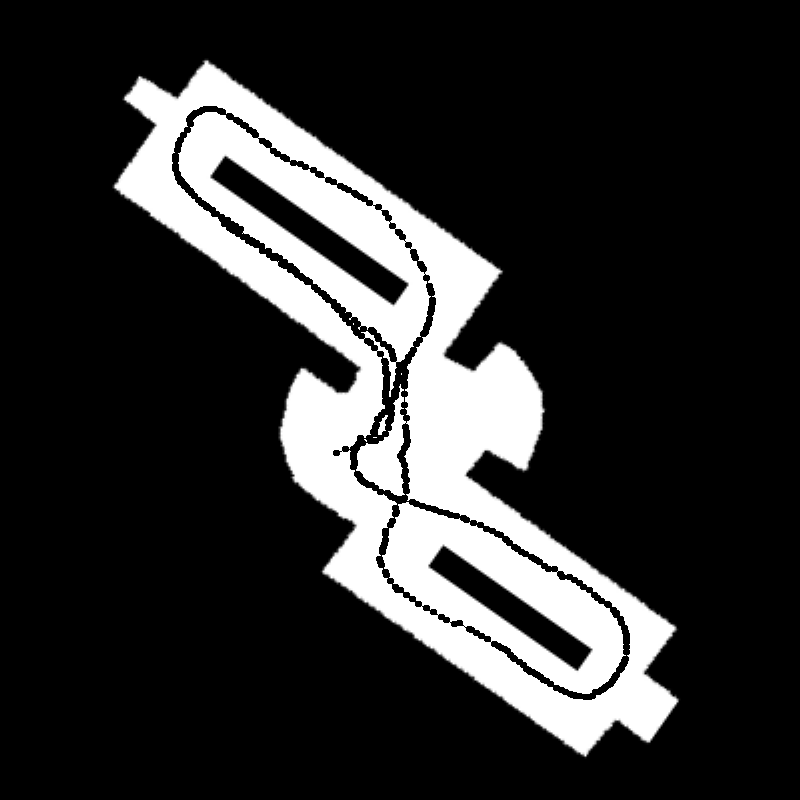
\includegraphics[scale=0.3]{hard-1.png}
	\end{subfigure}
	\begin{subfigure}
	\centering
	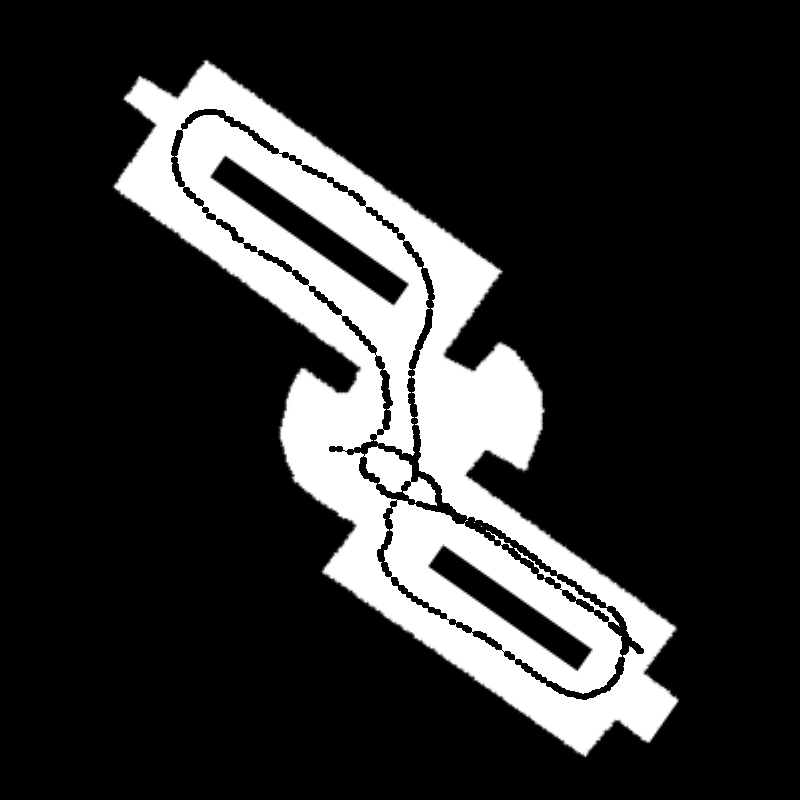
\includegraphics[scale=0.3]{hard-2.png}
	\end{subfigure}
\caption{The most likely trajectory in scenario ``hard'' from 5000 particle trajectories.}
\label{fig:hard}
\end{figure}

In the aforementioned two scenarios, there are three obstacles to localization. The minor ones are open space, where all sensors return the maximum readings, and symmetry in the map. The biggest obstacle to localization, though, is that there is only a small window around the global maximum (or its mirrors due to symmetry) where the likelihood is high enough to attract the distribution. This requires a relatively large initial population of particles to find. In practice, we tested 1000 and 5000 particles for scenario ``easy'', where 5000 particles lead to significantly better symmetry breaking in the early stage. For scenario ``hard'', we tested 2000 and 5000 particles, where the former scheme failed to find the global optimum at all. Therefore, we would conclude that if there are not sufficient particles, it is highly likely that the distribution would converge to an incorrect optimum.

\clearpage
\section{The Kidnapped Robot Problem}

A solution to the kidnapped robot problem is to add new, uniformly distributed particles at each step, hoping that some of them would be placed near the new global optimum (i.e. the new location of robot). However, such algorithm does not allow us to reconstruct the most likely trajectory. This is because in the kidnapping-free localization problem, all particles are created at the start of algorithm, so their history record starts from the first step. However, if we introduce new particles at later steps, there is no guarantee that at the end of the algorithm, any of the original particles could have survived the sequential sampling process. In other words, it is highly unlikely that we would not have a particle from which we can reconstruct the trajectory.

The key observation is that the kidnapped robot problem is equivalent to a piecewise kidnapping-free localization problem. Since the kidnapped robot is placed at an unknown place on the map, all we have to do is to identify the kidnapping, reconstruct the partial trajectory, and restart the algorithm. Here, we use the average weight of the best 10\% of particles to identify the kidnapping. When it falls below 0.001 (generally, this number is between 0.04 and 0.09), we assume that a kidnapping has happened. Using this method, we can see that the kidnapping happened at step 141, when the average weight dropped from 0.05319 to 0.0006777. The piecewisely reconstructed trajectory is shown in \hyperref[fig:kidnapped]{figure~\ref{fig:kidnapped}}, and the heatmap animation is available at \url{http://goo.gl/Pvgkgo}.

\hspace{2em}
\begin{figure}[htbp]
\centering

\includegraphics[scale=0.4]{kidnapped.png}
\caption{The most likely trajectory in scenario ``kidnapped'' from 5000 particle trajectories.}
\label{fig:kidnapped}
\end{figure}
\end{document}
